\documentclass{article}[12pt]
\usepackage{color}
\usepackage[normalem]{ulem}
\usepackage{times}
\usepackage{fullpage}
\usepackage{amsmath}
\usepackage{amssymb}
\usepackage{listings}
\usepackage{tikz}
\def \R {\mathbb R}
\def \imp {\Longrightarrow}
\def \eps {\varepsilon}
\def \Inf {{\sf Inf}}
\newenvironment{proof}{{\bf Proof.  }}{\hfill$\Box$}
\newtheorem{theorem}{Theorem}[section]
\newtheorem{definition}{Definition}[section]
\newtheorem{corollary}{Corollary}[section]
\newtheorem{lemma}{Lemma}[section]
\newtheorem{claim}{Claim}[section]
\setlength {\parskip}{2pt}
\setlength{\parindent}{0pt}

\newcommand{\headings}[4]{\noindent {\bf Final CME241} \hfill {{\bf Author:} Nicolas Sanchez} \\
{} \hfill {{\bf SUNETID:} sanchezn} \\

\rule[0.1in]{\textwidth}{0.025in}
}

\newcommand{\klnote}[1]{{\color{red} #1}}
\newcommand{\klsout}[1]{{\color{red} \sout{#1}}}

\begin{document}

\headings{\#1}{Tuesday, October 8, 10:30am}\section{} 



\section{Modified Shortest Path}
\subsection{Problem Formulation}
Suppose the grid given is of size $n\times m$, and that the terminal state set $\mathbf{T}$ and the set of blocks $\mathbf{B}$ are provided as given in the prompt. Then our state space will be defined as the coordinate pairs in the grid,  terminal states will be given trivially by $\mathbf{T}$ and non-terminal states  $\mathcal{N}$ will be states that are neither terminal nor blocked:

\begin{align*}
\mathcal{S} &= \{ (i,j) | i,j \in \mathbb{N}, 0\leq i \leq n-1, 0\leq j \leq m-1\}\\
\mathcal{T} &=\mathbf{T}\\
\mathcal{N} &= \{ (i,j) | (i,j) \in \mathcal{S}, (i,j)\not\in \mathbf{T}, (i,j) \not\in \mathbf{B}\}\\
\end{align*}

The actions for a given state will depend on the surrounding blocks but will be drawn from the set 

$$\mathbf{A} = \{(v,h) | v,h \in \{0,1,-1\}, |v|+|h| = 1\}$$

where intuitively $(0,1)$ is right, $(0,-1)$ left, $(1,0)$ up and $(-1,0)$ down. A given state will have all actions in $\mathbf{A}$ that do no lead to blocked or out of bound states, i.e. formally for any $(i,j)\in \mathcal{N}$:

$$ \mathcal{A}((i,j)) = \{(v,h) | v,h \in \mathbf{A}, (i+v, j+h) \in \mathcal{S}, (i+v, j+h) \not\in \mathcal{B}\}$$


We can now define transition probabilities (which will include rewards) by realising that we must take into account the possibility of wind moving away from an intended spot given the action if there are valid, non-blocked states above or below the intended move as well as the effect. Intuitively we realise we will transition to the intended next state ($(i+v, j+h)$) and not incur extra cost only if we move and the wind does not blow, so always with probability $1-p_{1,j+h}-p_{2,j+h}$. The remaining probability must then be spread to either different state outcomes (wind blows and there is a space to move into) or different rewards (wind blows but we bump). Formally for any $(i,j)\in\mathcal{N}, (v,h) \in \mathcal{A}((i,j)), (i',j')\in\mathcal{N}\cup\mathcal{T}$ (all combinations not stated have probability zero):

\begin{align}
P((i',j'), -1 | (v,h), (i,j)) &= \begin{cases} 1-p_{1,j'}-p_{2,j'} &\text{ if $i' = i+v, j' = j+h$}\\
p_{2,j'} & \text{ if $ i' = i+v+1, j' = j+h$}\\
p_{1,j'} & \text{ if $ i' = i+v-1, j' = j+h$}\end{cases}\\
P((i',j'),-1 -b | (v,h), (i,j))& =  p_{2,j'}\mathbb{I}_{(i'+1,j') \not\in \mathcal{N}\cup\mathcal{T}}+p_{1,j'}\mathbb{I}_{(i'-1,j') \not\in \mathcal{N}\cup\mathcal{T}} & \text{ if $i' = i+v, j' = j+h$}\\
\end{align}

Finally we, as suggested, use a discount factor of $\gamma = 1$.

\subsection{Implementation of MDP}
\begin{lstlisting}
    def get_transition_probabilities(self, nt_state: Cell) \
            -> Mapping[Move, Categorical[Tuple[Cell, float]]]:
        '''
        given a non-terminal state, return a dictionary whose
        keys are the valid actions (moves) from the given state
        and the corresponding values are the associated probabilities
        (following that move) of the (next_state, reward) pairs.
        The probabilities are determined from the wind probabilities
        of the column one is in after the move. Note that if one moves
        to a goal cell (terminal state), then one ends up in that
        goal cell with 100% probability (i.e., no wind exposure in a
        goal cell).
        '''
        d: Dict[Move, Categorical[Tuple[Cell, float]]] = {}
        for a, (r, c) in self.get_actions_and_next_states(nt_state):
            if (r, c) in self.terminals:
                d[a] = Categorical({((r, c), -1.): 1.})
            else:
                list_probs = {}

                # check if wind can blow
                has_up = (r+1 <self.rows) and ((r+1,c) not in self.blocks)
                has_down = (r > 0) and ((r-1,c) not in self.blocks)

                # probability of intended move (no wind)
                list_probs[((r,c),-1.)] = 1.-self.wind[c][0]-self.wind[c][1]

                # wind blows up no bump
                if has_up and self.wind[c][1] >0.0:
                    list_probs[((r+1,c),-1.)] = self.wind[c][1]
                
                # wind blows down no bump
                if has_down and self.wind[c][0] >0.0:
                    list_probs[((r-1,c),-1.)] = self.wind[c][0]
    
                # bump possibility!
                if not(has_up and has_down): 
                    list_probs[((r,c),-1.-self.bump_cost)] = \
                            self.wind[c][1]*(1-int(has_up))\
                                +self.wind[c][0]*(1-int(has_down))
                d[a] = Categorical(list_probs)
        return d
   \end{lstlisting}


\subsection{Implementation of SARSA Control with epsilon greedy}
\begin{lstlisting}
def get_sarsa_vf_and_policy(
        self,
        states_actions_dict: Mapping[Cell, Optional[Set[Move]]],
        sample_func: Callable[[Cell, Move], Tuple[Cell, float]],
        episodes: int = 10000,
        step_size: float = 0.01
    ) -> Tuple[V[Cell], FinitePolicy[Cell, Move]]:
        '''
        states_actions_dict gives us the set of possible moves from
        a non-block cell.
        sample_func is a function with two inputs: state and action,
        and with output as a sampled pair of (next_state, reward).
        '''
        q: Dict[Cell, Dict[Move, float]] = \
            {s: {a: 0. for a in actions} for s, actions in
             states_actions_dict.items() if actions is not None}
        nt_states: CellSet = {s for s in q}
        uniform_states: Choose[Cell] = Choose(nt_states)
        for episode_num in range(episodes):
            epsilon: float = 1.0 / (episode_num + 1)
            state: Cell = uniform_states.sample()
            '''
            write your code here
            update the dictionary q initialized above according
            to the SARSA algorithm's Q-Value Function updates.
            '''
            # go through a full episode
            action = self.epsilon_greedy_action(state, q,epsilon)
            while(True):
                next_state, reward = sample_func(state,action)
                
                # end while loop if end of road
                if(states_actions_dict[next_state] is None):
                    q[state][action] += step_size*(reward - q[state][action])
                    break

                next_action = self.epsilon_greedy_action(next_state, q,epsilon)
                q[state][action] += step_size*(
                    reward + q[next_state][next_action] - q[state][action])
                state = next_state
                action= next_action


        vf_dict: V[Cell] = {s: max(d.values()) for s, d in q.items()}
        policy: FinitePolicy[Cell, Move] = FinitePolicy(
            {s: Constant(max(d.items(), key=itemgetter(1))[0])
             for s, d in q.items()}
        )
        return (vf_dict, policy)
\end{lstlisting}

\subsection{Implementation of epsilon greedy off policy Q learning}
\begin{lstlisting}
def get_q_learning_vf_and_policy(
        self,
        states_actions_dict: Mapping[Cell, Optional[Set[Move]]],
        sample_func: Callable[[Cell, Move], Tuple[Cell, float]],
        episodes: int = 10000,
        step_size: float = 0.01,
        epsilon: float = 0.1
    ) -> Tuple[V[Cell], FinitePolicy[Cell, Move]]:
        '''
        states_actions_dict gives us the set of possible moves from
        a non-block cell.
        sample_func is a function with two inputs: state and action,
        and with output as a sampled pair of (next_state, reward).
        '''
        q: Dict[Cell, Dict[Move, float]] = \
            {s: {a: 0. for a in actions} for s, actions in
             states_actions_dict.items() if actions is not None}
        nt_states: CellSet = {s for s in q}
        uniform_states: Choose[Cell] = Choose(nt_states)
        for episode_num in range(episodes):
            state: Cell = uniform_states.sample()
            '''
            write your code here
            update the dictionary q initialized above according
            to the Q-learning algorithm's Q-Value Function updates.
            '''
           # go through a full episode
            action = self.epsilon_greedy_action(state, q,epsilon)
            while(True):
                next_state, reward = sample_func(state,action)
                
                # end while loop if end of road
                if(states_actions_dict[next_state] is None):
                    q[state][action] += step_size*(reward - q[state][action])
                    break

                next_action = self.epsilon_greedy_action(next_state, q,epsilon)
                q[state][action] += step_size*(
                    reward + max(q[next_state].values()) - q[state][action])
                state = next_state
                action= next_action
        vf_dict: V[Cell] = {s: max(d.values()) for s, d in q.items()}
        policy: FinitePolicy[Cell, Move] = FinitePolicy(
            {s: Constant(max(d.items(), key=itemgetter(1))[0])
             for s, d in q.items()}
        )
        return (vf_dict, policy)
\end{lstlisting}
\subsection{Results}
We include an image of the output of the code confirming that all three of the methods yield the same implicit/explicit optimal value functions and policies.

\begin{figure}
  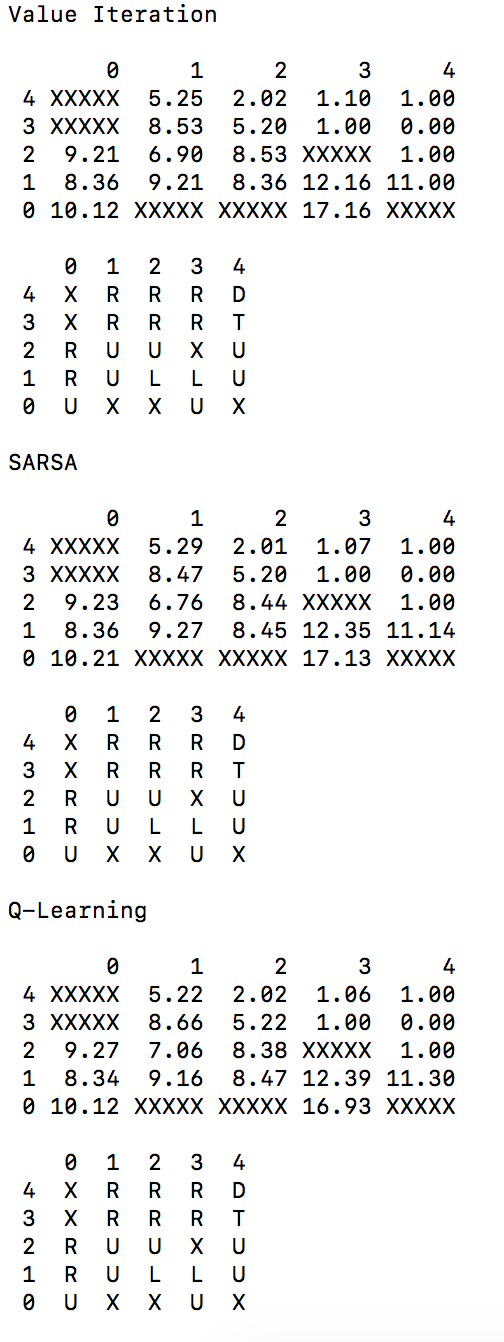
\includegraphics[width=0.5\linewidth]{CodeOutput.png}
  \caption{Convergence of three control methods}
  \label{fig:optPol1}
\end{figure}


\section{Discrete Time Constrained Consumption}
Let $x_0$ be the initial resource and $x_t$ be the remaining resource after $t$ discrete time steps. Since we are fixing $c = \theta x$ as the consumption at a given resource level $x$, we will have after $t$ time steps $x_t. = (1-\theta)^t x_0$. We can now plug that in to our known formula for the discounted aggregated utility:

\begin{align*}
V_\theta(x_0) &= \sum_{t=0}^{\infty} \beta^t U(\theta x_t)\\
&= \sum_{t=0}^{\infty} \beta^t U(\theta (1-\theta)^t x_0)\\
&= \sum_{t=0}^{\infty} \beta^t \frac{(\theta (1-\theta)^t x_0)^{1-\gamma}}{1-\gamma}\\
&= \frac{(\theta x_0)^{1-\gamma}}{1-\gamma}\sum_{t=0}^{\infty}  ((1-\theta)^{1-\gamma}\beta)^t \\
&= \frac{(\theta x_0)^{1-\gamma}}{1-\gamma}\frac{1}{1-(1-\theta)^{1-\gamma}\beta} \\
&= \frac{(\theta x_0)^{(1-\gamma)}}{(1-\gamma)(1-(1-\theta)^{1-\gamma}\beta)} \\
\end{align*}
Note that we are implicitly using the fact given in piazza that we assume a combination of $\gamma, \beta$ such that the sum converges.
We take the derivative with respect to $\theta$ to eventually find critical points:
\begin{align*}
\frac{\partial V_\theta (x_0)}{\partial \theta} &= \frac{x_0^{(1-\gamma)}(1-\gamma)\theta^{-\gamma}}{(1-\gamma)(1-(1-\theta)^{1-\gamma}\beta)}- \frac{x_0^{(1-\gamma)}(1-\gamma)\theta^{1-\gamma}(1-\theta)^{-\gamma}\beta}{(1-\gamma)(1-(1-\theta)^{1-\gamma}\beta)^2} \\
&= \frac{x_0^{(1-\gamma)}\theta^{-\gamma}(1-(1-\theta)^{1-\gamma}\beta)}{(1-(1-\theta)^{1-\gamma}\beta)^2}- \frac{x_0^{(1-\gamma)})\theta^{1-\gamma}(1-\theta)^{-\gamma}\beta}{(1-(1-\theta)^{1-\gamma}\beta)^2} \\
&= \frac{x_0^{(1-\gamma)}\theta^{-\gamma}[1-(1-\theta)^{1-\gamma}\beta - \theta (1-\theta)^{-\gamma}\beta]}{(1-(1-\theta)^{1-\gamma}\beta)^2} \\
&= \frac{x_0^{(1-\gamma)}\theta^{-\gamma}[1-(1-\theta)^{-\gamma}\beta(1-\theta + \theta)]}{(1-(1-\theta)^{1-\gamma}\beta)^2} \\
&= \frac{x_0^{(1-\gamma)}\theta^{-\gamma}[1-(1-\theta)^{-\gamma}\beta]}{(1-(1-\theta)^{1-\gamma}\beta)^2} \\
\end{align*}

We now note that this can be zero only if either $\theta = 0$ or $1-(1-\theta)^{-\gamma}\beta =0$ which would yield $$\theta^* =1 - \beta^{1/\gamma}$$

Note that since $x_0, \gamma > 0$ the sign of $\frac{\partial V_\theta (x_0)}{\partial \theta}$ will be the sign of $1-(1-\theta)^{-\gamma}\beta$ which is positive for $0<\theta < \theta^*$ and negative for $\theta^*<\theta < 1$ meaning that that $V_{\theta^*}(x_0)$ is indeed maximal. 

Plugging this back into the value function we get:
$$ V_{\theta^*}(x_0) =\frac{((1 - \beta^{1/\gamma}) x_0)^{(1-\gamma)}}{(1-\gamma)(1-(\beta^{1/\gamma})^{1-\gamma}\beta)} = \frac{((1 - \beta^{1/\gamma}) x_0)^{(1-\gamma)}}{(1-\gamma)(1-\beta^{1/\gamma})}$$

We note in particular that:


\begin{align*}
V_{\theta^*}(x_0) - \beta V_{\theta^*}((1-\theta^*)x_0) &= \frac{((1 - \beta^{1/\gamma}) x_0)^{(1-\gamma)}}{(1-\gamma)(1-\beta^{1/\gamma})} - \beta \frac{((1 - \beta^{1/\gamma}) \beta^{1/\gamma} x_0)^{(1-\gamma)}}{(1-\gamma)(1-\beta^{1/\gamma})}\\
&= \frac{((1 - \beta^{1/\gamma}) x_0)^{(1-\gamma)} [1 - \beta(\beta^{1/\gamma})^{1-\gamma}]}{(1-\gamma)(1-\beta^{1/\gamma})} \\
&= \frac{((1 - \beta^{1/\gamma}) x_0)^{(1-\gamma)} (1 - \beta^{1/\gamma}))}{(1-\gamma)(1-\beta^{1/\gamma})} \\
&= \frac{((1 - \beta^{1/\gamma}) x_0)^{(1-\gamma)}}{(1-\gamma)} \\
&= U(\theta^* x_0) \\
\end{align*} 

And since $V_\theta^*(x_0) = U(\theta^* x_0) + \beta V_\theta^*((1-\theta)x_0)$ is exactly the bellman recursive equation so we have validated that our optimal policy and value satisfy the bellman equation. We also have:


\begin{align*}
U(\theta x) + \beta V_{\theta^*}((1-\theta)x) &= \frac{(\theta x)^{1-\gamma}}{1-\gamma} + \beta\frac{((1 - \beta^{1/\gamma}) (1-\theta)x)^{(1-\gamma)}}{(1-\gamma)(1-\beta^{1/\gamma})}\\
 &= \frac{x^{(1-\gamma)}(\theta^{1-\gamma}(1-\beta^{1/\gamma}) +\beta((1 - \beta^{1/\gamma}) (1-\theta))^{(1-\gamma)})}{(1-\gamma)(1-\beta^{1/\gamma})}\\
  &= \frac{x^{(1-\gamma)}(1-\beta^{1/\gamma})(\theta^{1-\gamma} +\beta(1 - \beta^{1/\gamma})^{-\gamma} (1-\theta)^{(1-\gamma)})}{(1-\gamma)(1-\beta^{1/\gamma})}\\
\end{align*}
Maximising this is the same as maximising $M(\theta) = \theta^{1-\gamma} +\beta(1 - \beta^{1/\gamma})^{-\gamma} (1-\theta)^{(1-\gamma)}$. We take the derivative:
\begin{align*}
\frac{\partial M(\theta)}{\partial \theta} &= (1-\gamma)\theta^{-\gamma} - \beta(1-\gamma)(1 - \beta^{1/\gamma})^{-\gamma}(1-\theta)^{-\gamma}
\end{align*}
And setting this to zero yields:
\begin{align*}
\theta^{-\gamma} &= \beta(1 - \beta^{1/\gamma})^{-\gamma}(1-\theta)^{-\gamma}\\
\theta&= \beta^{-1/\gamma}(1 - \beta^{1/\gamma})(1-\theta)\\
\theta&=( \beta^{-1/\gamma} - 1)(1-\theta)\\
\theta(1+ \beta^{-1/\gamma} - 1)&=\beta^{-1/\gamma} - 1\\
\theta&=1- \beta^{1/\gamma} = \theta^*\\
\end{align*}
Note that $\frac{\partial^2 M(\theta)}{\partial \theta^2} = -\gamma (1-\gamma)\theta^{-\gamma-1} - \beta(1-\gamma)\gamma (1-\beta^{1/\gamma})(1-\theta)^{-1-\gamma}$ is always negative since $\gamma>0, \theta,\beta \in [0,1]$ so $\theta^*$ is maximising $M(\theta)$ and hence $U(\theta x) + \beta V_{\theta^*}((1-\theta)x)$
Hence we do have
$$V_{\theta^*}(x) = \max_\theta\{ U(\theta x) + \beta V_{\theta^*}((1-\theta)x) \} $$
where the equality comes from our validation of the bellman equation earlier, and the maximisation at policy $c^* = \theta^*x$ was just proven so we have validated the Bellman optimality equation.

\section{Mortgage Switch MDP}
\subsection{Problem Formulation}
We construct the MDP formulation as follows, assuming the functions for balance remaining, interest payments, principal payments given in the prompt ($B_i(L,M), I_i(L,M), P_i(L,M)$). The state is completely determined by the loan amount, loan rate and time since inception of existing loan $i_t$ as well as the offered new rate $N$ and absolute time $t$ (month and year).
$$ \mathcal{S} = \{(L,M, i_t, t, N) | L, M, N \in \mathbb{R}, t,i_t \in \mathbb{N_+}\}$$ 

The actions at any state are given as strings representing taking or not taking offer for the new loan rate (and amount):

$$\mathcal{A} = \{\text{"ACCEPT"}, \text{"PASS"}\}$$
 
The reward is given by making the payments on the existing loan and rate and potential transaction cost:

$$ R( (L',M', i_t', t', N'), a,  (L,M, i_t, t, N)) = -P_{i_t}(L,M) - I_{i_t}(L,M)-C\mathbb{I}_{a = \text{"ACCEPT"}}$$

The transition probabilities are given based on $\mathbf{N}_{t}$ which is the random variable representing the offered mortgage rate on month/year $t$. All combinations not represented have probability zero.

\begin{align*}
P((L,M, i_t+1, t+1, N')| \text{"PASS"}, (L,M,i_t,t, N)) = Pr(\mathbf{N}_t = N')\\
P((B_{i_t+1}(L,M),N, 0,t+1, N')| \text{"ACCEPT"}, (L,M,i_t, t, N)) = Pr(\mathbf{N}_{t} = N')\\
\end{align*}

With the specified annual rate we set the discount factor over each discrete time period (month) to be:

$$ \gamma = (1+r)^{-1/12}$$
\subsection{Solution Approach}
In the problem formulation described above, the economist would essentially give us access to sample the random variables $\mathbf{N}_t$ we expect to see in coming years. With this in hand, we can simulate the MDP and resulting MRPs for a given policy. In particular for any pair $(L,M,i_t,t,N)$ and action we would be able to sample the next step $(L,M,i_t+1, t+1,N')$ by sampling $N'$ from $\mathbf{N}_t$ if the action is to decline the offer or $(B_i(L,M),N, 0,t+1, N')$ again by doing the computations and sampling $N'$ from $\mathbf{N}_t$.

A few consideration when choosing the RL approach. We notice that the time dependence of the problem means that episodic analysis could prove useful in capturing underlying dynamics. Also, since we have access to the actual stochastic process, we can generate as many simulations as possible so we are not constrained by lack of data and have the ability to generate episodes. As such we like the idea of using eligibility traces (TD($\lambda$)) objectives to combine the robustness of convergence of MC and the reduced variance of TD errors.\\

Intuitively, the problem naturally places importance both on the decision making and the inherent value of a state. Notably, our ultimate goal is to be able to recommend or follow a given policy without necessarily caring about the value it is suggesting. That being said, the setup of the problem suggests that really the key in making the right decision is recognizing the value of a given mortgage offer using future expected potential mortgage rates you may get and your current mortgage situation. To balance this dual importance of our problem we see the Actor Critic as the best model as it simultaneously learns the value and policy.

We propose an Actor Critic with Eligibility Traces to attack the problem. More specifically we model both the policy and value function as dense neural networks with three layers each. For the features we will use an augmented version of the state to include intuitively important state features:
$$(B_{i_t}(L,M), I_{i_t}(L,M), P_{i_t}(L,M), L, M, N, i_t, t)$$

The first two layers will be shared by both models and have 100 neurons each to allow for learning of potentially complicated relationships. The Actor will have a final layer of two neurons with softmax output activation which will correspond to the probability of accepting or rejecting. The Critic will have a final layer of one with no output activation and this will be the value of a given state.

We will use the Actor Critic Eligibility trace algorithm as presented in class for the training (Algorithm 4.3), initially setting both $\lambda$ parameters to $0.5$ before doing some parameter searching to find the optimal combination. We initially use Adam optimization for decreasing learning rates and use $\epsilon$-greedy policies with $\epsilon$ exponentially decaying as we see more and more episodes to encourage exploration of the large space.

This approach makes use of the availability of data and has the potential to capture many possible functional forms using a broad function approximation with neural networks. The main risk is the introduction of bias as well as potential running time to convergence on the model. The hope is that the bias vs computation can be handled by toggling the $\lambda$ parameter as necessary and perhaps more or less deep neural networks are needed.

\end{document}
